\chapter{Transmissão dos dados em série}\label{chap:chap4}

Este capítulo aborda o trabalho realizado na segunda parte do projeto, tal como definido em ~\ref{sec:descrição_objetivos}. Esta parte do projeto consiste em transmitir em paralelo para o transmissor GTX existente na FPGA VC7203 que ,através da sua arquitetura, serializa os dados e envia-os através de um cabo físico. Esse mesmo cabo conectado ao recetor GTX irá deserializar para que sejam convertidos novamente para dados em paralelo.

Este processo de serialização e deserialização exige muitos cuidados e aplicações de determinados métodos que permitam manter a integridade do sinal durante a transmissão do mesmo, já como explicado em no capítulo 2 em \ref{serial_theory}. Todavia nesse mesmo capítulo, em \ref{sub:arqGTX} foi já abordado que FPGA VC7203 possui entradas e saídas de alta velocidade com arquiteturas que possuem blocos que permitem a implementação destes mecanismos. Na imagem \ref{fig:gtx_geral_arq} da página \pageref{fig:gtx_geral_arq} visualiza-se uma arquitetura geral dos transcetores, mas estes serão descritos com mais detalhe neste capítulo.

Este capítulo começa por abordar as arquiteturas transmissora e recetora com mais detalhe e quais as características que são vantajosas a este projeto. De seguida serão contempladas as arquiteturas desenvolvidas e explicadas todas as decisões no seu desenvolvimento.

\section{Transmissor} \label{sec:tx_gtx}

Na figura \ref{fig:gtx_tx_arq} da página \pageref{fig:gtx_tx_arq} visualiza-se a arquitetura do transmissor GTX. Assim como já foi mencionado, esta arquitetura possui muitos blocos com diferentes funções que permitem manter a integridade do sinal durante uma transmissão, pelo menos, daquilo que se pode fazer do lado do transmissor.
\begin{figure}[h!]
	\begin{center}
		\leavevmode
		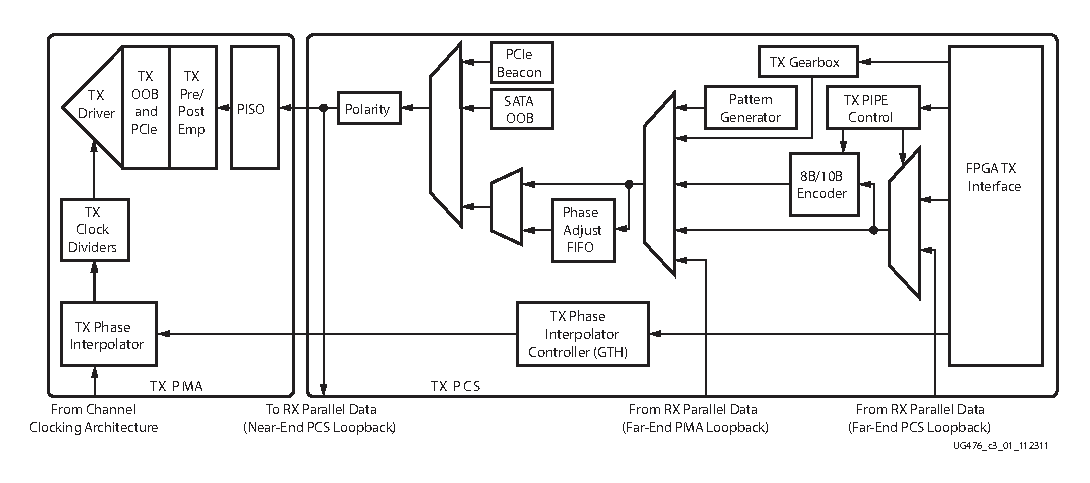
\includegraphics[width=1.0\textwidth]{tx_gtx_arq}
		\caption{Arquitetura do transmissor GTX, retirada de \cite{R011}}
		\label{fig:gtx_tx_arq}
	\end{center}
\end{figure}

Os blocos mais relevantes para o funcionamento do projeto passam de seguida a ser descritos nas próxima subsecções para que se possa entender mais facilmente as arquiteturas desenvolvidas quando estas forem apresentadas.

\subsection{Interface com a FPGA} \label{subch:tx_interface}

Na imagem \ref{fig:gtx_tx_arq} este bloco tem o nome de "\textit{FPGA TX Interface}" e é o bloco por onde entram os dados em paralelo provenientes da FPGA que se pretendem serializar. Segundo \cite{R011}, o tamanho desta interface depende de vários fatores internos, como por exemplo, o tamanho interno que os dados terão (pode estar dependente da utilização de codificação) e ainda o tamanho do \textit{datapath} que se escolhe usar.

%%Tamanho das interfaces
Para se perceber melhor como o tamanho da porta desta interface pode variar é apresentada a table \ref{table:tx_interface} na página \pageref{table:tx_interface} que expõe os casos possíveis.


\begin{table}[h!]
	\centering
	\resizebox{\textwidth}{!}{%
		\begin{tabular}{rlll}
			\hline
			\multicolumn{1}{c}{\textbf{Codificação 8B/10B}} & \multicolumn{1}{c}{\textbf{Tamanho do \textit{datapath}}} & \multicolumn{1}{c}{\textbf{Tamanho Interno}} & \multicolumn{1}{c}{\textbf{Interface com a FPGA}} \\ \hline
			\multicolumn{1}{r|}{Sim}                        & 0 (2 byte)                                       & 20                                           & 16                                                \\
			\multicolumn{1}{r|}{Sim}                        & 0 (2 byte)                                       & 20                                           & 32                                                \\
			\multicolumn{1}{r|}{Sim}                        & 1 (4 byte)                                       & 40                                           & 32                                                \\
			\multicolumn{1}{r|}{Sim}                        & 1 (4 byte)                                       & 40                                           & 64                                                \\
			\multicolumn{1}{r|}{Não}                        & 0 (2 byte)                                       & 16                                           & 16                                                \\
			\multicolumn{1}{r|}{Não}                        & 0 (2 byte)                                       & 20                                           & 20                                                \\
			\multicolumn{1}{r|}{Não}                        & 0 (2 byte)                                       & 16                                           & 32                                                \\
			\multicolumn{1}{r|}{Não}                        & 1 (4 byte)                                       & 32                                           & 32                                                \\
			\multicolumn{1}{r|}{Não}                        & 0 (2 byte)                                       & 20                                           & 40                                                \\
			\multicolumn{1}{r|}{Não}                        & 1 (4 byte)                                       & 40                                           & 40                                                \\
			\multicolumn{1}{r|}{Não}                        & 1 (4 byte)                                       & 32                                           & 64                                                \\
			\multicolumn{1}{r|}{Não}                        & 1 (4 byte)                                       & 40                                           & 80                                                \\ \hline
		\end{tabular}%
	}
	\caption{Tamanhos possíveis para a interface da FPGA com o GTX transmissor, adaptada de \cite{R011}}
	\label{table:tx_interface}
\end{table}

Os diferentes tamanhos que a porta da interface pode tomar estão apresentados na última coluna da tabela tendo em conta que quando é implementada uma codificação então estes apenas podem variar entre 16, 32 ou 64. Todavia quando não há codificação, então o tamanho desta porta pode ser os valores anteriormente referidos ou então até mesmo 20,40 ou 80. De notar que quando não há codificação e o tamanho da porta é 16, 32 ou 64 existe a possibilidade de extender esses valores (caso se pretenda) para 20, 40 e 80 respetivamente. No entanto, tal não será abordado dado que não é importante para o projeto. 

Os valores do tamanho interno do \textit{datapath} podem variar entre 2 e 4 bytes, contudo é necessário tomar em atenção que quando um \textit{datapath} de um determinado tamanho não chega para o número de bits à entrada então é necessário utilizar dois. Mas isto será abordado mais à frente nesta subsecção. 

%%Relógios que saem e para que servem
Os dados em paralelo entram neste bloco a uma determinada cadência bem definida : ao flanco positivo do sinal de relógio \textit{TXUSRCLK2}. Este sinal de relógio é o sinal de sincronização entre os dados provenientes da FPGA com o transmissor, no entanto é também necessário outro sinal de relógio para a lógica interna PCS do transmissor : \textit{TXUSRCLK}. De recordar que a lógica interna PCS trabalha com os dados em paralelo ainda e portanto o valor deste sinal de relógio vai depender não só da cadência a que os dados em paralelo (\textit{TXUSRCLK2}) entram no transmissor mas também do \textit{datapath} escolhido.

Por um lado, o sinal de relógio \textit{TXUSRCLK2} é o principal sinal de sincronização entre a lógica da FPGA e a lógica do transmissor, por outro o sinal de relógio \textit{TXUSRCLK} é a cadência determinista dos dados em paralelo no bloco PCS, e por isso existe uma relação entre estes dois sinais muito bem definida que passa a ser apresentada na tabela \ref{table:freq_tx} na página \pageref{table:freq_tx}.

\begin{table}[h!]
	\centering
	\resizebox{\textwidth}{!}{%
		\begin{tabular}{lll}
			\hline
			\multicolumn{1}{c}{\textbf{Tamanho na Interface}} & \multicolumn{1}{c}{\textbf{Tamanho do \textit{datapath}}} & \multicolumn{1}{c}{\textbf{Relação entre os sinais de relógio}} \\ \hline
			16, 20 (bits)                                     & 0 (2 byte)                                       & $F_{TXUSRCLK} = F_{TXUSRCLK2}  $                                    \\
			32, 40 (bits)                                     & 0 (2 byte)                                       & $F_{TXUSRCLK} = F_{TXUSRCLK2} * 2$                                  \\
			32, 40 (bits)                                     & 1 (4 byte)                                       & $F_{TXUSRCLK} = F_{TXUSRCLK2} $                                      \\
			64, 80 (bits)                                     & 1 (4 byte)                                       & $F_{TXUSRCLK} = F_{TXUSRCLK2} * 2$                                  \\ \hline
		\end{tabular}%
	}
	\caption{Relação entre as frequências dos sinais de relógio \textit{TXUSRCLK2} e \textit{TXUSRCLK}, adaptada de \cite{R011}}
	\label{table:freq_tx}
\end{table}


%Explicar que se pode obter uma estimativa da velocidade de transmissão de acordo com aquela equação
Segundo \cite{R011}, sabendo estas relações entre os sinais de relógio, o tamanho da porta na interface do transmissor e o tamanho do \textit{datapath} usado é possível obter a velocidade de transmissão do dados em série através da equação apresentada em \ref{eq:lineRate} na página \pageref{eq:lineRate}.

\begin{equation} \label{eq:lineRate}
Line\ Rate = F_{TXUSRCLK}*(Internal\ Datapath\ Width)
\end{equation}


%Explicar pq e que tem frequências diferentes visto que sao os dois para sinais em paralelo
Para que se perceba a diferença entre estas frequências é agora apresentado um caso em concreto que é utilizado neste projeto: pretende-se na entrada do transmissor obter 40 bits em paralelo, ou seja, ter uma porta com uma largura de 40 bits, e que estes dados sejam amostrados a uma frequência de 148,5 MHz ($F_{TXUSRCLK2} = 148,5\ MHz$). Assim sendo, existem agora duas hipóteses: a utilização de um \textit{datapath} de 2 byte ou 4 byte.

Se se optar pela utilização de um \textit{datapath} de 4 byte então está-se perante a opção a), ilustrada na imagem \ref{fig:exemplo_datapaths} da página \pageref{fig:exemplo_datapaths}, em que o sinal de amostragem à entrada é de 148,5 MHz ($F_{TXUSRCLK2} = 148,5\ MHz$) e o sinal de lógica do bloco PCS também é 148,5 MHz ($F_{TXUSRCLK} = 148,5\ MHz$), tal como ilustrado na figura. Neste caso a largura do sinal interno é de 40 bits o que, segundo a equação \ref{eq:lineRate}, perfaz uma taxa de saída do sinal serializado de $5,94\ Gb/s$.

Se por outro lado, se optar por um \textit{datapath} interno de 2 byte, então serão necessários 2 \textit{datapaths}, tal como ilustra o caso b) da figura \ref{fig:exemplo_datapaths}. Isto implica que a taxa de amostragem nesses sejam o dobro da cadência de entrada dos sinais na interface com transmissor. Assim, mantém-se uma frequência de amostragem à entrada do transmissor de $F_{TXUSRCLK2} = 148,5\ MHz$ e uma frequência do sinal de relógio de cada bloco PCS de $F_{TXUSRCLK} = 297\ MHz$. Ou seja, a largura interna de cada datapath é de 20 bits e por isso a taxa de saída do sinal serializado será igual a $5,94\ Gb/s$, segundo a equação \ref{eq:lineRate}.

\begin{figure}[h!]
 	\begin{center}
 		\leavevmode
 		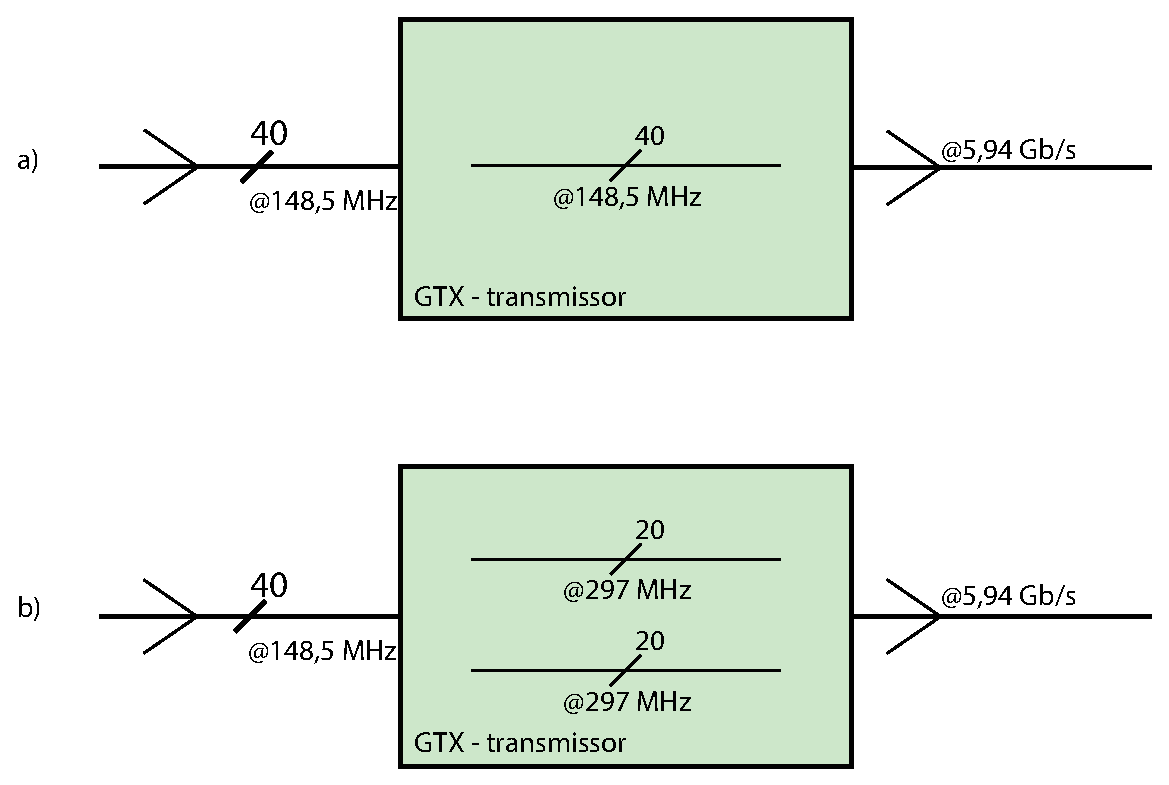
\includegraphics[width=0.75\textwidth]{exemplo_datapath}
 		\caption{Exemplo simplificado de transmissão com diferentes usos de \textit{datapath}}
 		\label{fig:exemplo_datapaths}
 	\end{center}
 \end{figure}

%%Concluir como se geram estes sinais
Estes dois sinais de relógio são gerados neste bloco e colocados nas saídas do mesmo para que na FPGA possa ser desenvolvida uma arquitetura que leia os sinais em paralelo para o transmissor à cadência de \textit{TXUSRCLK2}. Estes estão alinhados pelo flanco positivo dos mesmos ainda que tenham frequências diferentes. Ambos são gerados com base no sinal de relógio de referência, segundo \cite{R011} e \cite{R022}, através de multiplicadores ou divisores caso possuam frequências diferentes.


\subsection{Codificador 8B/10B}

Este bloco permite que os sinais em paralelo sejam codificados de 8 bits para 10 bits quando está ativo. Por outras palavras, através da codificação extende os sinais de entrada de 16 bits para 20 bits, os sinais de 32 bits para 40 bits e os sinais de 64 bits para 80 bits. É de notar que apesar de ser vantajosa a utilização de codificação num protocolo de transmissão em série, que a ativação deste bloco aumenta a latência do transmissor, tal como é de esperar.

As características deste tipo de codificação, as suas vantagens e importância foram já abordadas na subsecção com o título "Codificação dos sinais e sua importância" em \ref{subsub:cod_impor} no capítulo \ref{chap:chap2}.

\subsection{Gerador de padrões pseudo-aleatórios}

A geração de sequência pseudoaleatórias é bastante utilizada em sistemas de telecomunicações para testar a integridade do sinal de ligações de grande velocidade, segundo \cite{R011}. Apesar de estas mesmas sequências parecerem aleatórias à primeira vista, na realidade apresentam determinadas características que são utilizadas para medir a qualidade da ligação. Este bloco do transmissor é responsável por esta ação. 

\subsection{\textit{Driver} do Transmissor}

\subsection{Interface com a camada física}

\section{Recetor} \label{sec_rx_gtx}

\begin{figure}[h!]
	\begin{center}
		\leavevmode
		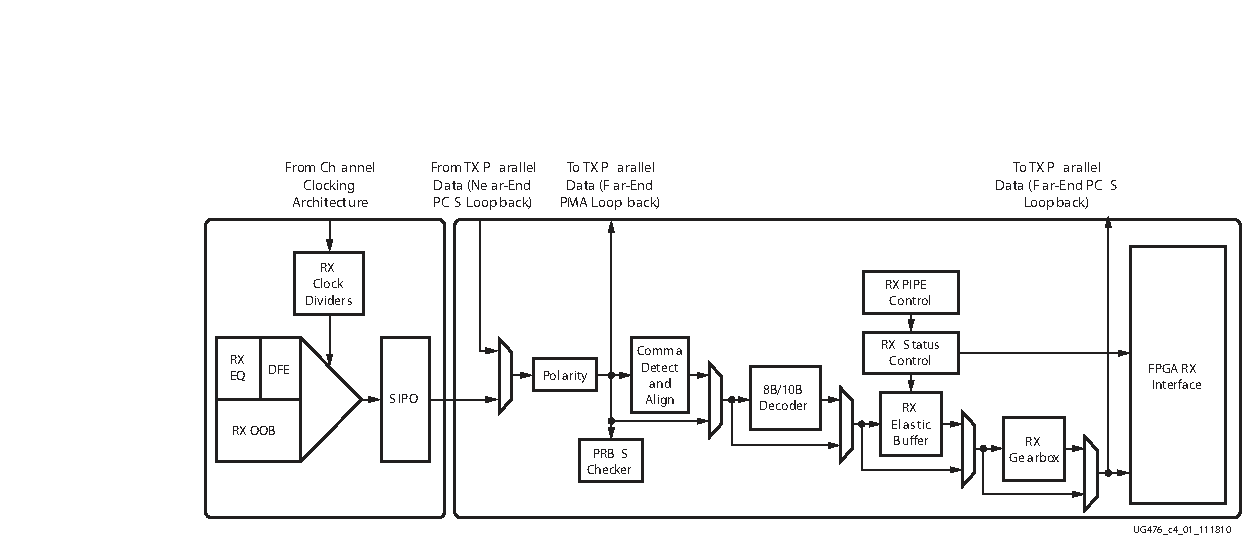
\includegraphics[width=1.0\textwidth]{rx_gtx_arq}
		\caption{Arquitetura do recetor GTX, retirada de \cite{R011}}
		\label{fig:gtx_rx_arq}
	\end{center}
\end{figure}	

\subsection{Analog Front-End}	
	
\subsection{Equalização}

\subsection{CDR}

\subsection{Pattern Checker}

\subsection{Byte and Word Alignament}

\subsection{Elastic Buffer}

\subsection{Clock Correction}

\subsection{Interface com a FPGA}
	
\section{Estrutura dos pacotes}

\section{Velocidades de transmissão possiveis de alcançar no projeto}

\section{Arquitetura para formar tramas}

\section{Estr}

\section{Arquitetura para recuperar as tramas}
	
	
	
	
	
	
	
	
	
	
	
	
	%Em \cite{R031} é sugerido que o valor do sinal de relogio de referencia seja o mesmo proveninete da fonte HDMI isto porque a frequência o sinal de relógio de referência deve ser exatamente igual (ou multiplo) da cadência dos dados de entrada.